\subsection{SRGAN}

El SISR (Single Image Super Resolution) es un problema inverso, \emph{it est}, que para una imagen de baja resolución puede haber muchas
imágenes diferentes de alta resolución que le correspondan, esto basado en la interpretación del método utilizado, ya que
el principio básico es añadir información para obtener imágenes de alta resolución.
Las CNN presentan un gran avance en la reconstrucción de imágenes de baja resolución a alta resolución,
sin embargo, debido al escalado de la imagen o el hecho de que la imagen que se busca mejorar presenta grandes
variaciones con respecto a las del dataset (\emph{Data Augmentation}) los resultados podrían ser no satisfactorios.


Una alternativa que propone un nuevo paradigma son las GAN´s (Generative Adversarial Networks), cuyo funcionamiento está basado
en la estimación de modelos generadores, como mencionan Goodfellow et al. \cite{GANs}, esto es 
posible gracias al entrenamiento simultáneo de dos modelos, uno \emph{generador (G)} que obtiene 
la distribución de la entrada para generar datos falsos y el otro \emph{discriminador (D)} el cual se encarga de estimar 
la probabilidad de que la muestra provenga del dataset de entrenamiento y discernir así entre estos datos y 
los del modelo \emph{ generador (G)}.

El término \emph{antagónicas} como se menciona en \cite{SRGAN_Tesis}, se refiere a la dinámica 
competitiva que se mantiene entre los dos modelos. Por un lado,
el generador tiene por objetivo crear nuevos datos que sean indistinguibles del
conjunto de entrenamiento, mientras que el discriminador debe poder ser capaz
de distinguir cuáles son los datos creados y los reales, siendo los últimos los que corresponden
 al conjunto de entrenamiento como se ve en la imagen \ref{Alexis1}. Esto resulta en un proceso iterativo donde estos dos modelos
 se desafían uno a otro, logrando un ajuste de parámetros
 que logran producir datos que se parezcan con gran acierto a los reales.
 

\begin{figure}[H]
    \begin{center}
      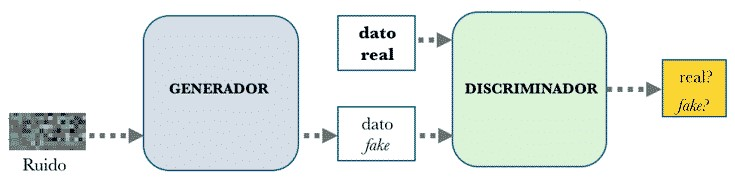
\includegraphics[scale = 0.7]{GANmodelo.jpg}
      \caption{Enfoques del Modelo Generador y Discriminador}
      \label{Alexis1}
    \end{center}
\end{figure}


El modelo SRGAN (Super Resolution Generative Adversarial Network) fue
propuesto en 2016 por un grupo de investigadores de la empresa Twitter \cite{SRGAN}.
La principal innovación de este modelo es su función de pérdida, llamada
función de pérdida perceptual, que permite mejorar el realismo de la imagen de
salida.

\subsubsection{Componentes.}

Profundizando un poco más en los componentes del algoritmo, en especifico, el uso de las \emph{GAN´s} para la obtención de Super-Resolución (\emph{SRGAN}), 
tenemos al discriminador el cual es una red neuronal convolucional que consta de muchas 
capas ocultas y una capa de salida, la principal diferencia aquí es que la capa de salida de las GAN puede tener solo dos salidas, 
a diferencia de las CNN, que pueden tener un número diferente de salidas con respecto a la cantidad de etiquetas en las que está entrenado.
La salida del discriminador puede ser 1 o 0 dependiendo de la función de activación que se aplique. Si la salida es 1, 
entonces los datos proporcionados son reales y si la salida es 0, entonces se refiere a ellos como datos falsos como se ve en la imagen \ref{Alexis2}.

El discriminador está capacitado con los datos del dataset, con estos aprende a reconocer cómo se ven y qué características deben 
clasificarse como reales, formalmente, discrimina entre $\tilde{x}$, la muestra falsa, y $x$, 
los datos muestreados de la distribución real de datos $P_{datos}(x)$.




\begin{figure}[H]
    \begin{center}
      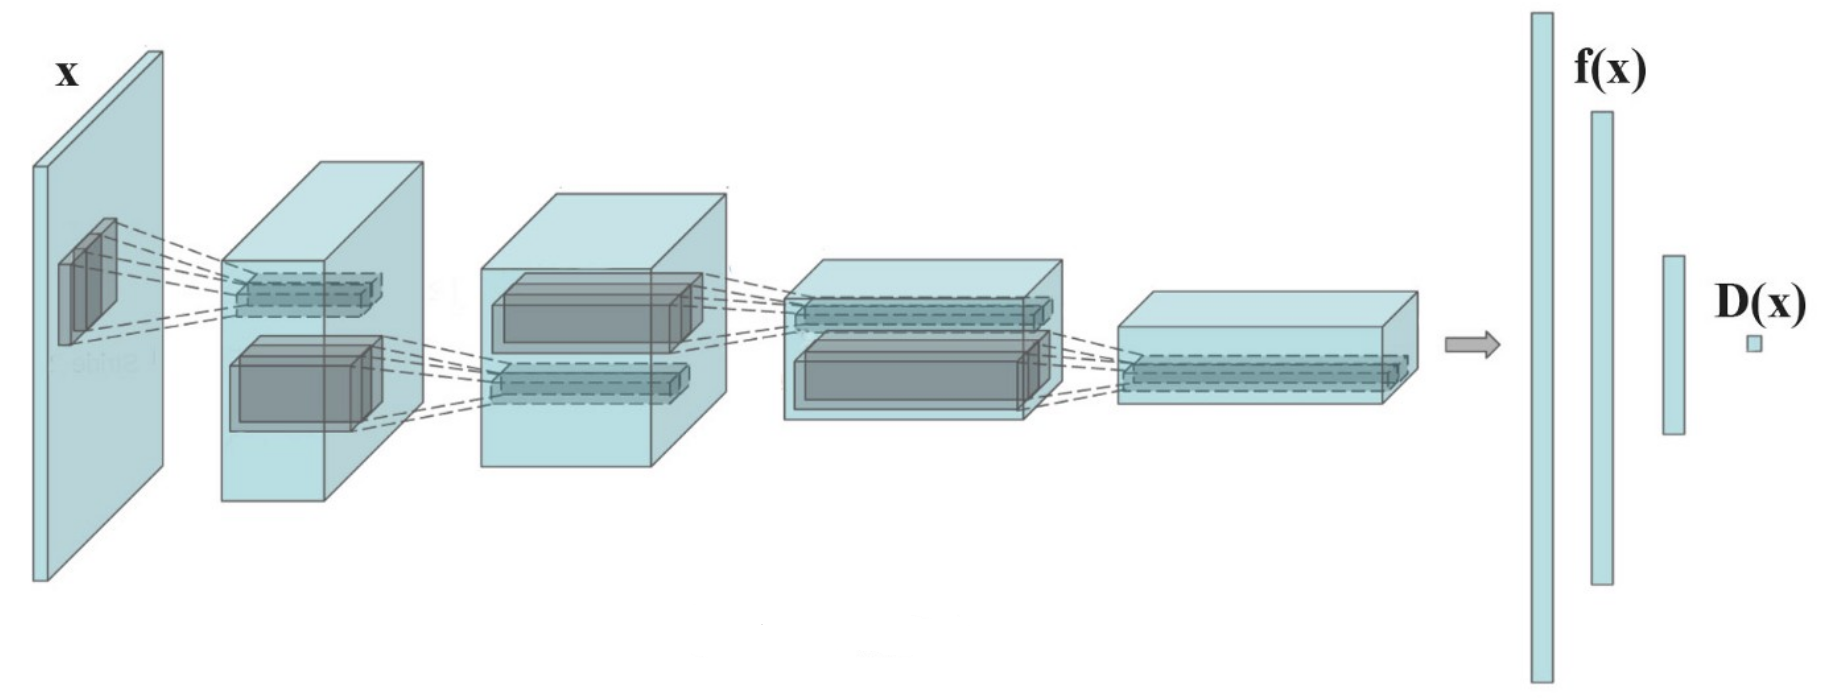
\includegraphics[scale = 0.4]{discriminador.png}
      \caption{Modelo Discriminador}
      \label{Alexis2}
    \end{center}
\end{figure}


Por el contrario, el generador es una red neuronal convolucional inversa, hace exactamente lo opuesto de lo que hace una CNN, ya que 
a estas se les da una imagen real como entrada y se espera una etiqueta clasificada como salida, 
pero en el generador, un vector de ruido aleatorio\emph{(z)} se da como señal de entrada 
y se espera una imagen falsa como salida, esta imagen deberá aproximarse a la real a
partir de una distribución $P(z)$ (en general una distribución Gaussiana) que
produce una muestra de datos falsos,$\tilde{x}$ como se muestra en la imagen \ref{Alexis3}

\begin{equation}
G(z) = \tilde{x}
\end{equation}

\begin{figure}[H]
    \begin{center}
      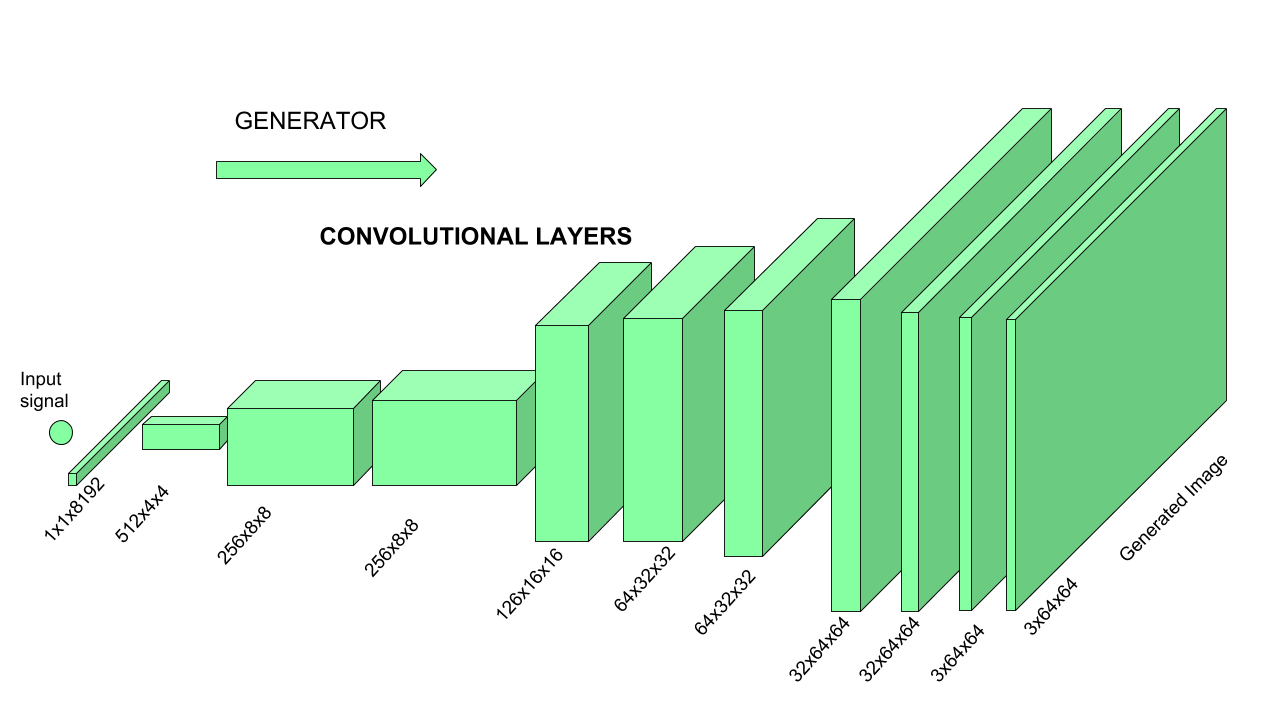
\includegraphics[scale = 0.6]{generador.png}
      \caption{Modelo Generador}
      \label{Alexis3}
    \end{center}
\end{figure}
    
\subsubsection{Funciones de perdida.}

Como parte del entrenamiento se necesitan parámetros que nos describan de manera correcta los resultados
que obtenemos de la predicción en nuestra red neuronal, para esto se hace el uso de funciones de perdida, estas funciones 
evalúan la desviación entre las predicciones realizadas por la red neuronal y los valores 
reales de las observaciones utilizadas durante el aprendizaje. A esta función se le conoce como perdida perceptual. Cuanto menor es el resultado de esta función, 
más eficiente es la red neuronal. Su minimización, es decir, reducir al mínimo la desviación entre el valor de la predicción y
el valor real para una observación dada, se hace ajustando los distintos pesos de la red neuronal.

En el caso de las redes adversarias, específicamente en \emph{SRGAN}, esta perdida es la suma de las perdidas de contenido $l_{X}^{SR}$ 
y las adversarias $10^{-3}l_{Gen}^{SR}$.


\begin{equation}
  l^{SR}=l_{X}^{SR} + 10^{-3}l_{Gen}^{SR}
\end{equation}


Como mencionan Goodfellow et al. \cite{GANs}, se tienen 
2 perdidas principales: La de contenido (\emph{content loss}), la cual se aproxima a una perdida perceptual mediante la perdida
de la red neuronal (\emph{VGG}),definimos entonces la perdida \emph{VGG} como la distancia euclidiana entre la representación de
características de una imagen reconstruida $G_{\theta G}(l^{LR})$ y la imagen de referencia o real $l^{HR}$.


\begin{equation}
  l_{VGG/i.j}^{SR}=\frac{1}{W_{i,j}H_{i,j}} \sum_{x=1}^{W_{i,j}}\sum_{y=1}^{H_{i,j}}(\phi_{i,j}(l^{HR})_{x,y}-\phi_{i,j} 
  (G_{\theta G}(l^{LR}))_{x,y})^{2}
\end{equation}

Por otra parte tenemos la perdida adversaria, esta se añade el componente generador de nuestro modelo GAN a la perdida perceptual,
esto promueve que nuestra red cree soluciones que engañen al discriminador. Las perdidas del generador $l_{Gen}^{SR}$ se definen
en base a las probabilidades del modelo discriminador $D_{\theta D}(G_{\theta G}(l^{LR}))$ sobre las muestras de entrenamiento
de la siguiente manera:

\begin{equation}
  l_{Gen}^{SR}=\sum_{n=1}^{N}-log \ D_{\theta D}(G_{\theta G}(l^{LR}))
\end{equation}


Donde $D_{\theta D}(G_{\theta G}(l^{LR}))$ es la probabilidad de que nuestra imagen reconstruida $G_{\theta G}(l^{LR})$ sea 
una imagen de alta resolución y la función logarítmica nos ayuda con el comportamiento del gradiente. 

Las GANs presentan varios desafíos a eludir durante su entrenamiento
que son actualmente temas de investigación. Entre ellos, los problemas más
usuales que surgen en el entrenamiento de una GAN son:

\begin{itemize}


    \item No convergencia:El generador y el discriminador no logran alcanzar un equilibrio. La
función de pérdida del generador y discriminador empiezan a oscilar sin
poder lograr a largo plazo una estabilidad.
Si bien es común en las GAN que en un comienzo las funciones de pérdida
oscilen, a medida que transcurre el entrenamiento el objetivo es que se
logre una estabilidad. Cuando esto no ocurre, las muestras son producidas
por el generador, pero su calidad no mejora.

\item Colapso modal:Esto ocurre cuando el generador produce muestras similares aunque las
entradas sean de muy diversas características. El generador encuentra que
un conjunto pequeño de muestras engañan al discriminador y entonces
no es capaz de producir otras. En estos casos, el gradiente de la función
de pérdida queda estancado en un valor cercano a 0.

\item Pérdida no informativa: Aunque parezca natural pensar que cuanto menor sea la pérdida del
generador, mayor será la calidad de las muestras que produce, esto no
resulta tan inmediato. La pérdida del generador debe ser comparada con
la del discriminador, que se encuentra en constante mejora. Por lo tanto,
no es tan sencillo evaluar la mejora del modelo. El generador podría estar
produciendo muestras cada vez de mayor calidad, aun cuando la función
de pérdida se vaya incrementando.

\end{itemize}
